\chapter{Documentación de las nuevas funciones} \label{chp:anexo_docs_funcs}

En este anexo se puede encontrar la documentación generada para cada nueva función propuesta a la librería \pvlibpy{}. Se incluye en forma de imágenes, solo el cuerpo con el contenido relevante, para poder apreciar el resultado que vería un usuario final.

Si se desea ver el código fuente de la documentación, en el caso de las propuestas aceptadas basta con acceder al link de la función y pinchar en el botón \textit{[source]}. Para el caso de las no aceptadas, habría que acceder a la \gls{rama} de trabajo de la propuesta mediante la \textit{\gls{pull request}} correspondiente.

%%%%%%%%%%%%%%%%%%%%%%%%%%%%%%%%%%%%%%%%%%%%%%%%%%%%%%%%%%%%%%%%%%%%%%%%%%%%%%%%
\begin{myparindent}{0pt}

\newpage\section{Modelo de ajuste espectral} \label{sct:doc_modelo_nuria}

Propuesta en \pr{1658}, no aceptada.

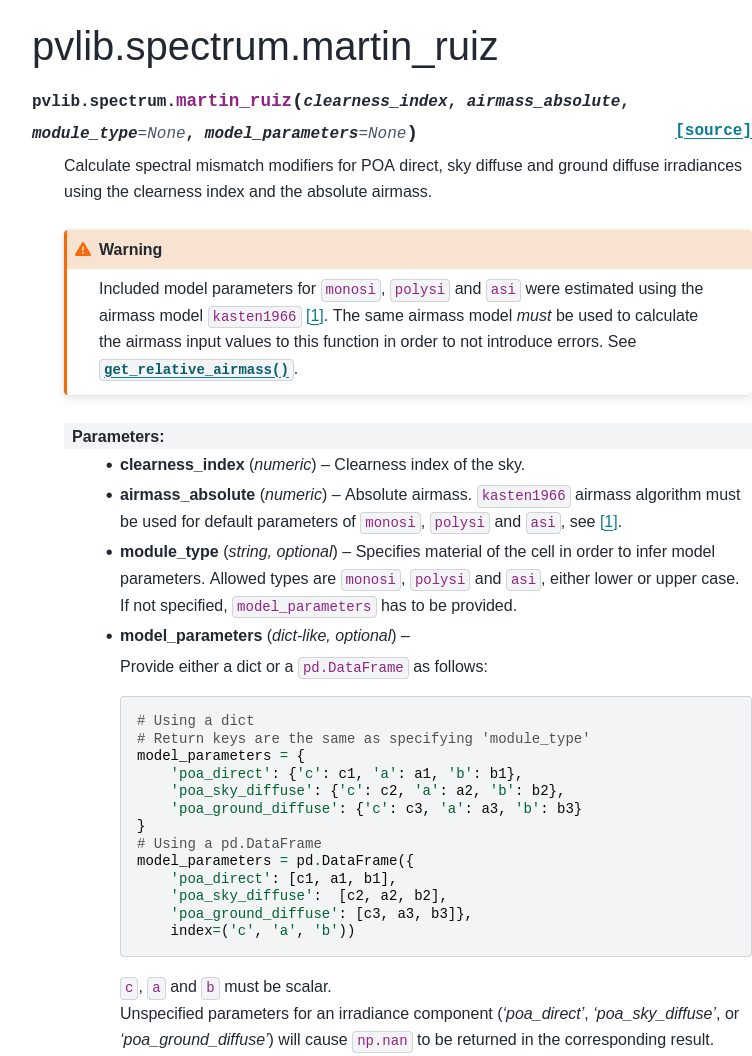
\includegraphics[width=\linewidth,height=0.9\textheight,keepaspectratio]{images/docs_funcs_cut/martin_ruiz_0.png}

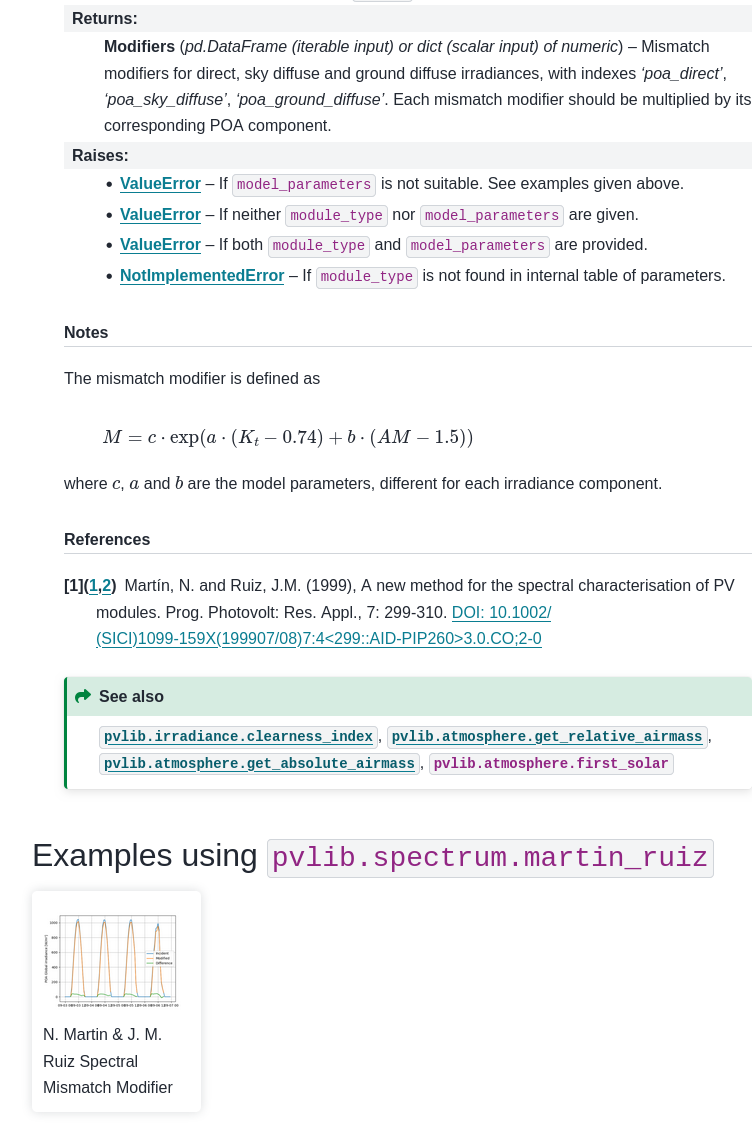
\includegraphics[width=\linewidth,height=0.9\textheight,keepaspectratio]{images/docs_funcs_cut/martin_ruiz_1.png}

\newpage\section{Proyección del cenit solar} \label{sct:doc_proyeccion_cenit}

\pr{1904}, accesible en \linkDocsFunction{pvlib.shading.projected\_solar\_zenith\_angle}.

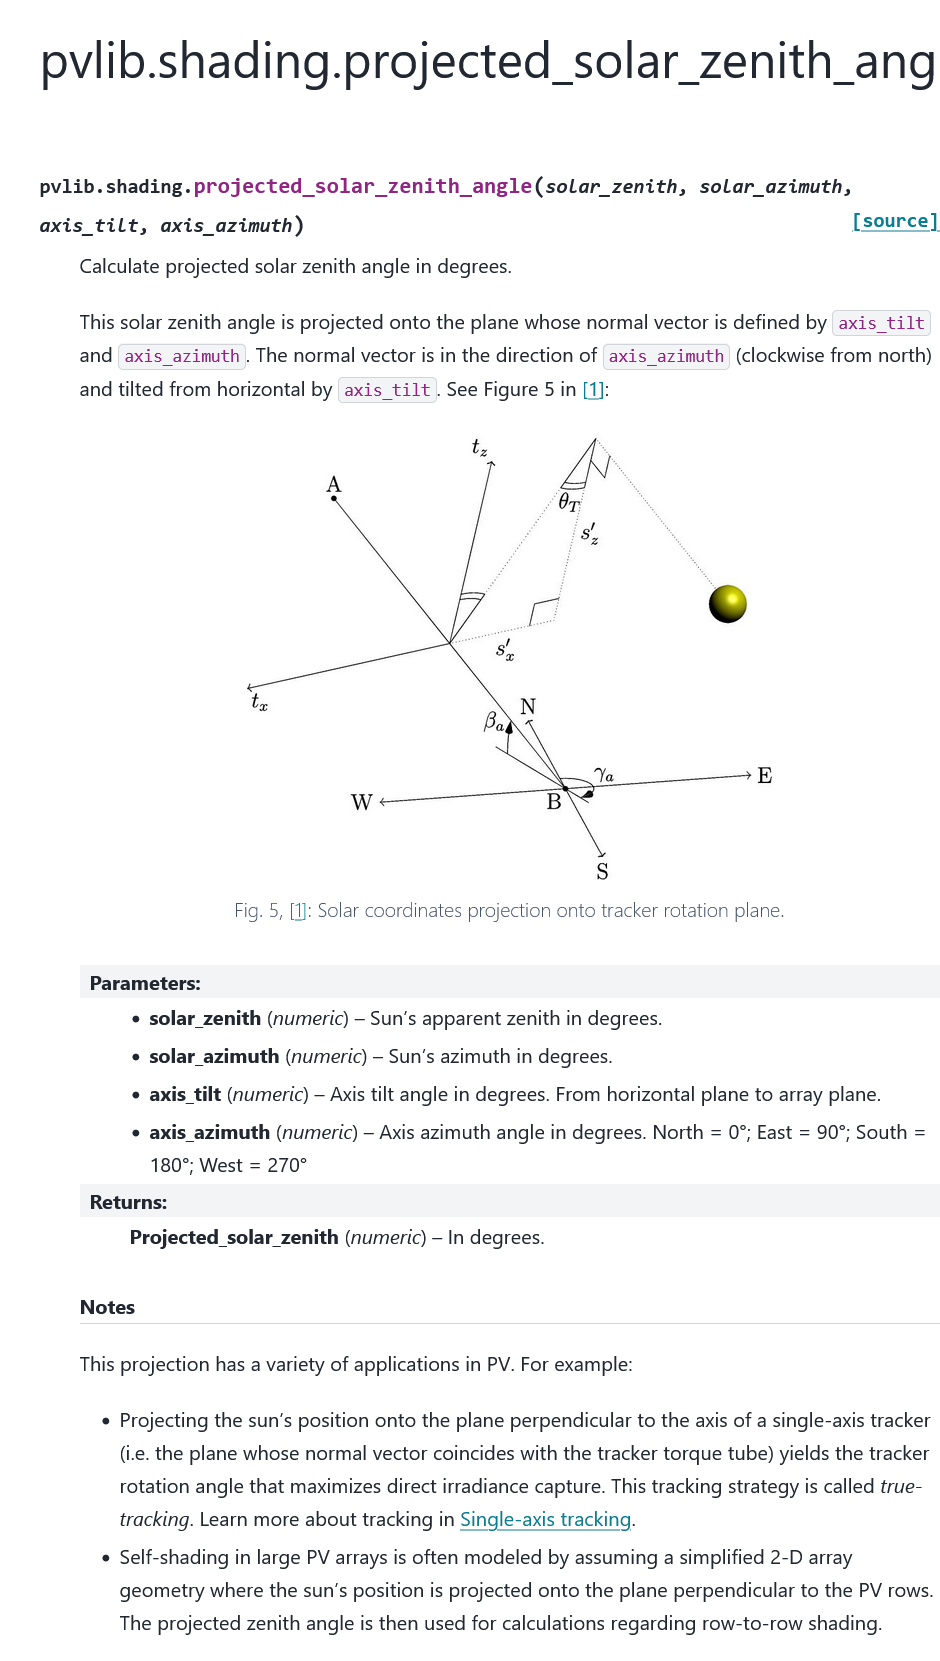
\includegraphics[width=\linewidth,height=0.9\textheight,keepaspectratio]{images/docs_funcs_cut/projected_solar_zenith_angle_0.png}

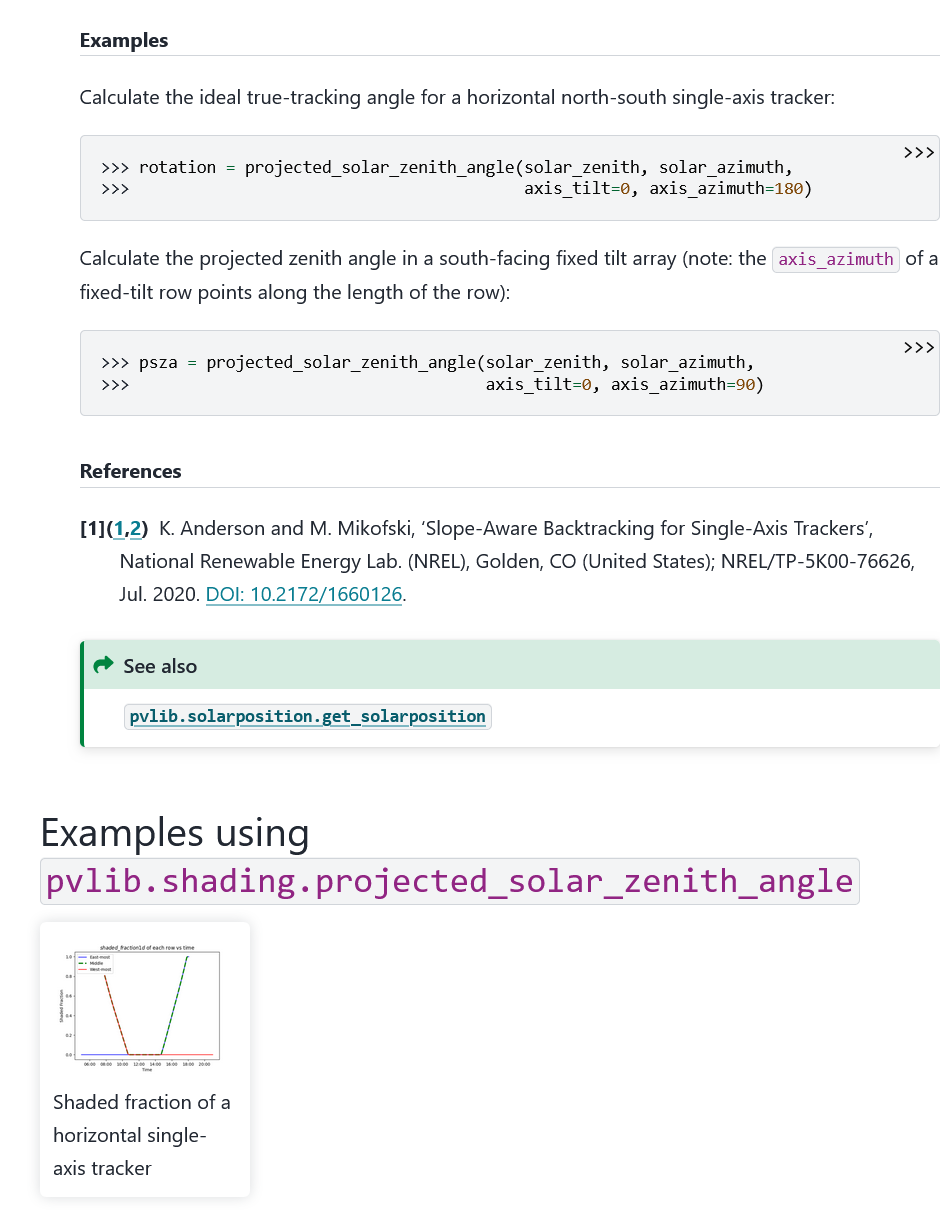
\includegraphics[width=\linewidth,height=0.9\textheight,keepaspectratio]{images/docs_funcs_cut/projected_solar_zenith_angle_1.png}

\newpage\section{Fracción de sombra unidimensional} \label{sct:doc_fraccion_sombra}

\pr{1962}, accesible en \linkDocsFunction{pvlib.shading.shaded\_fraction1d}.

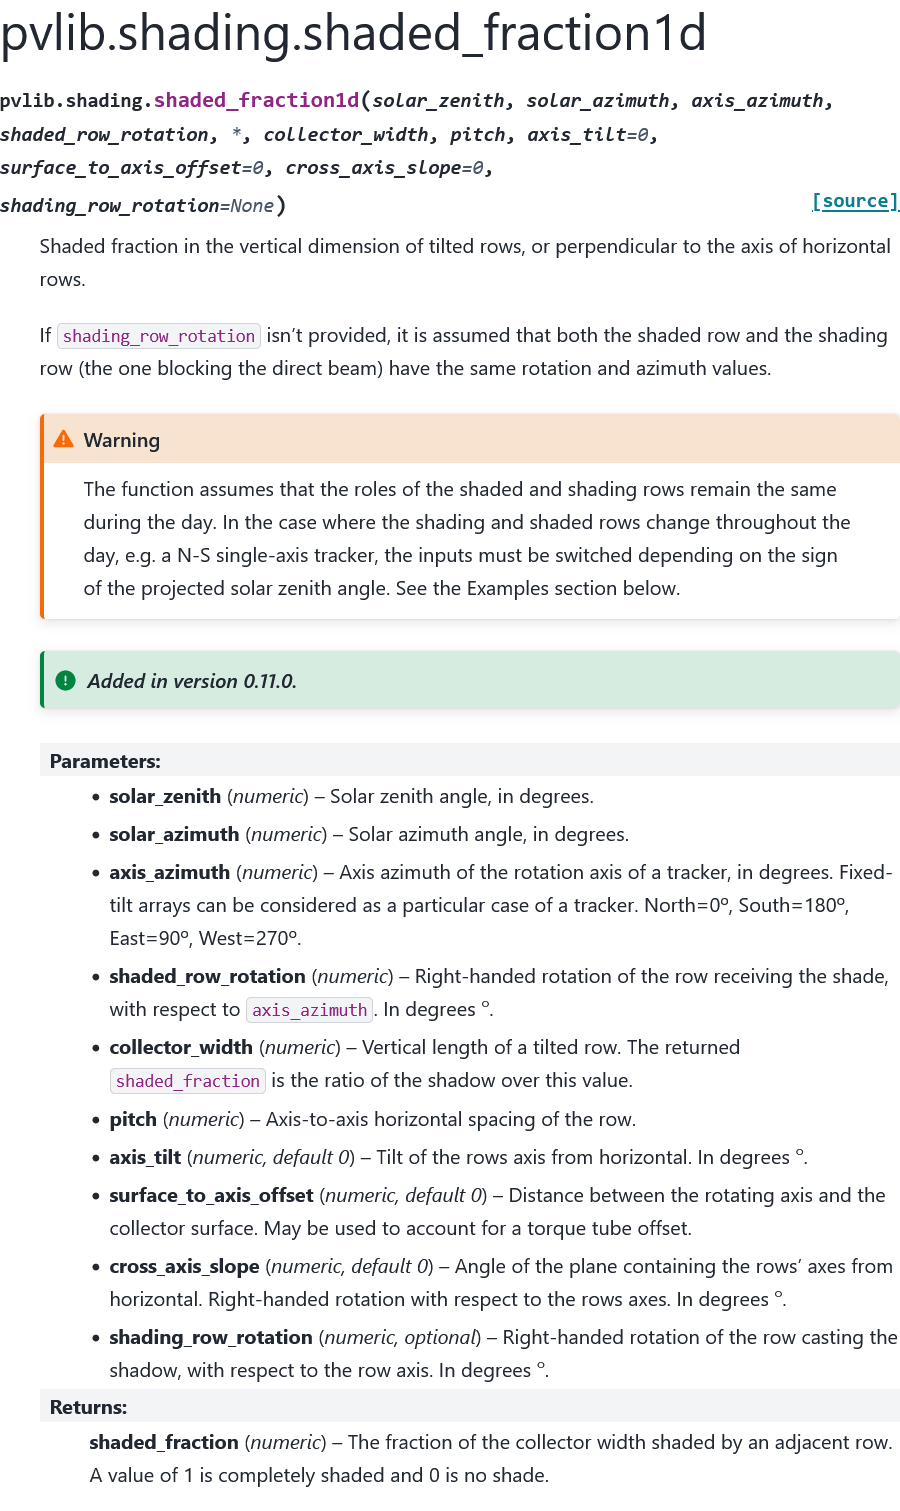
\includegraphics[width=\linewidth,height=0.9\textheight,keepaspectratio]{images/docs_funcs_cut/shaded_fraction1d_0.png}

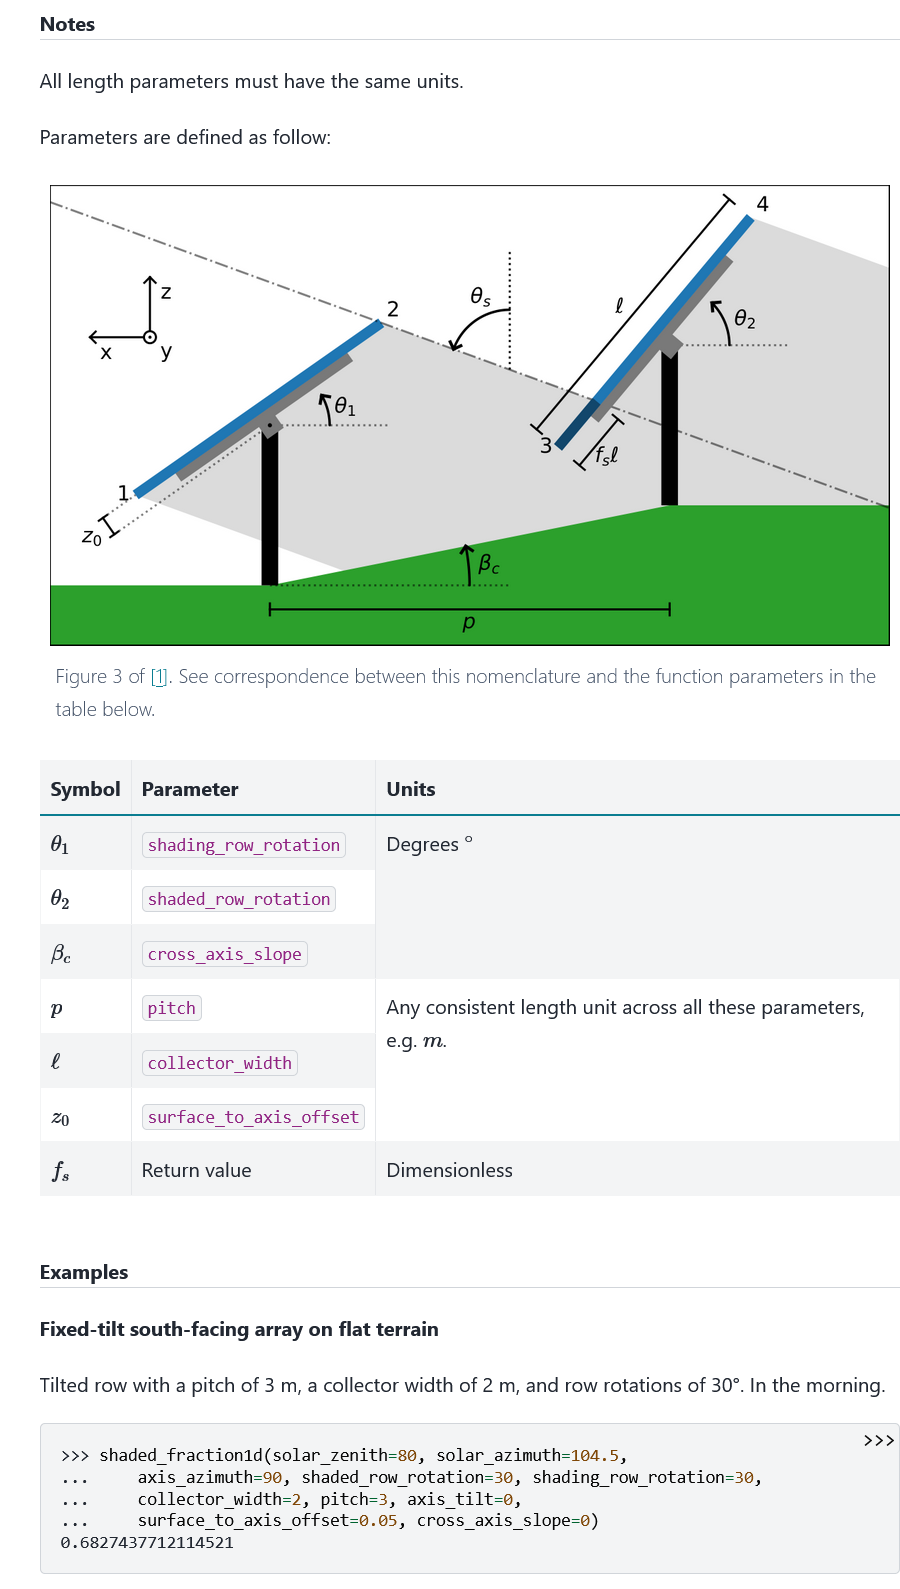
\includegraphics[width=\linewidth,height=0.9\textheight,keepaspectratio]{images/docs_funcs_cut/shaded_fraction1d_1.png}

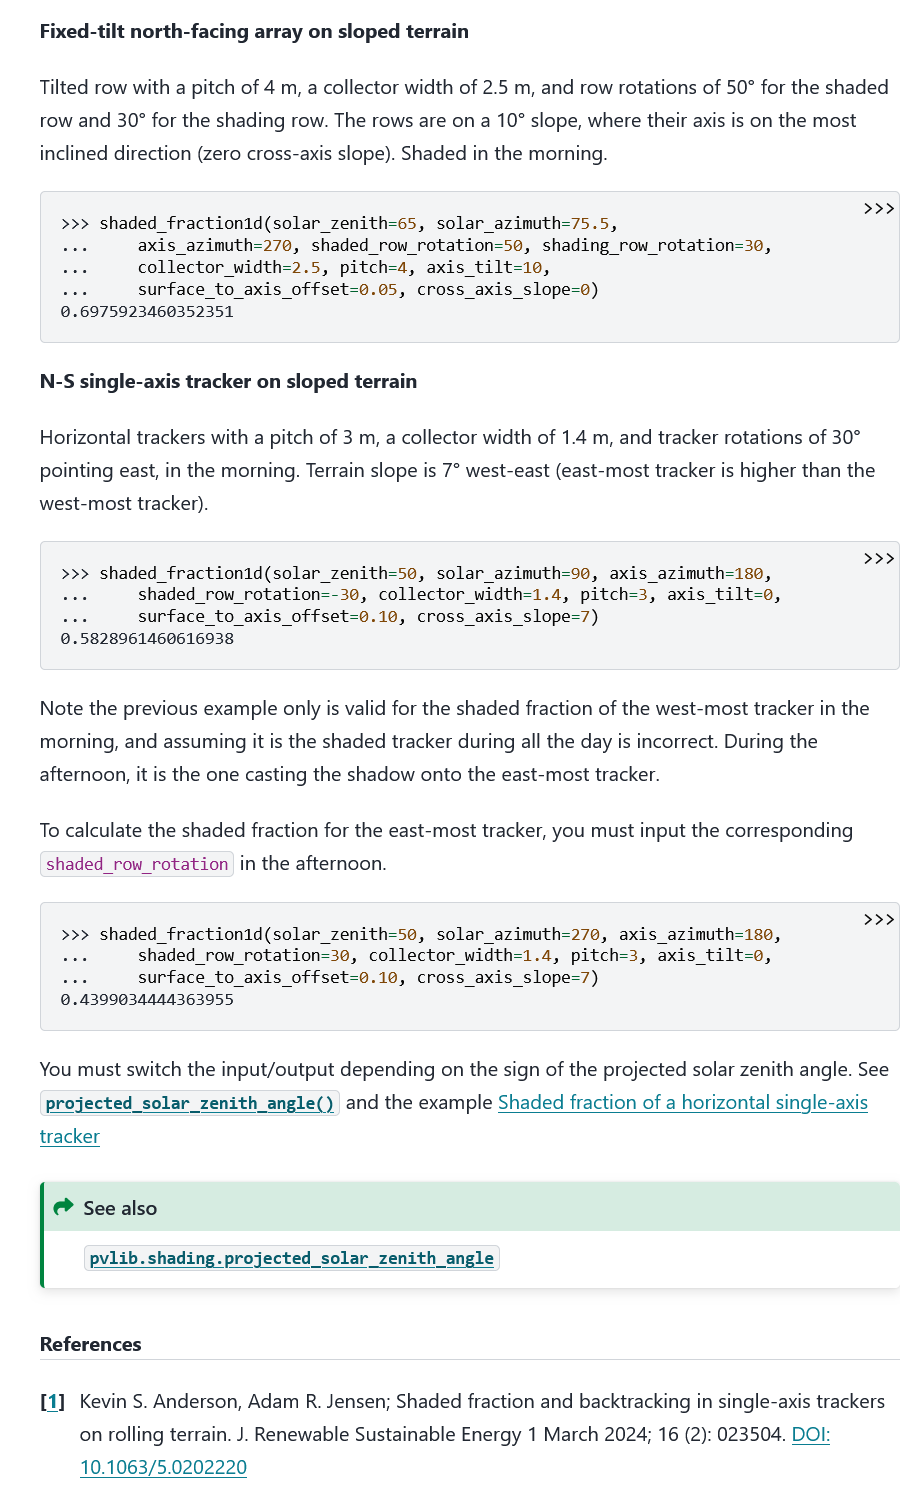
\includegraphics[width=\linewidth,height=0.9\textheight,keepaspectratio]{images/docs_funcs_cut/shaded_fraction1d_2.png}

\newpage\section{Pérdidas por sombras en módulos con diodos de bypass} \label{sct:doc_modelo_perdidas_sombra}

\pr{2070}, accesible en \linkDocsFunction{pvlib.shading.direct\_martinez}.

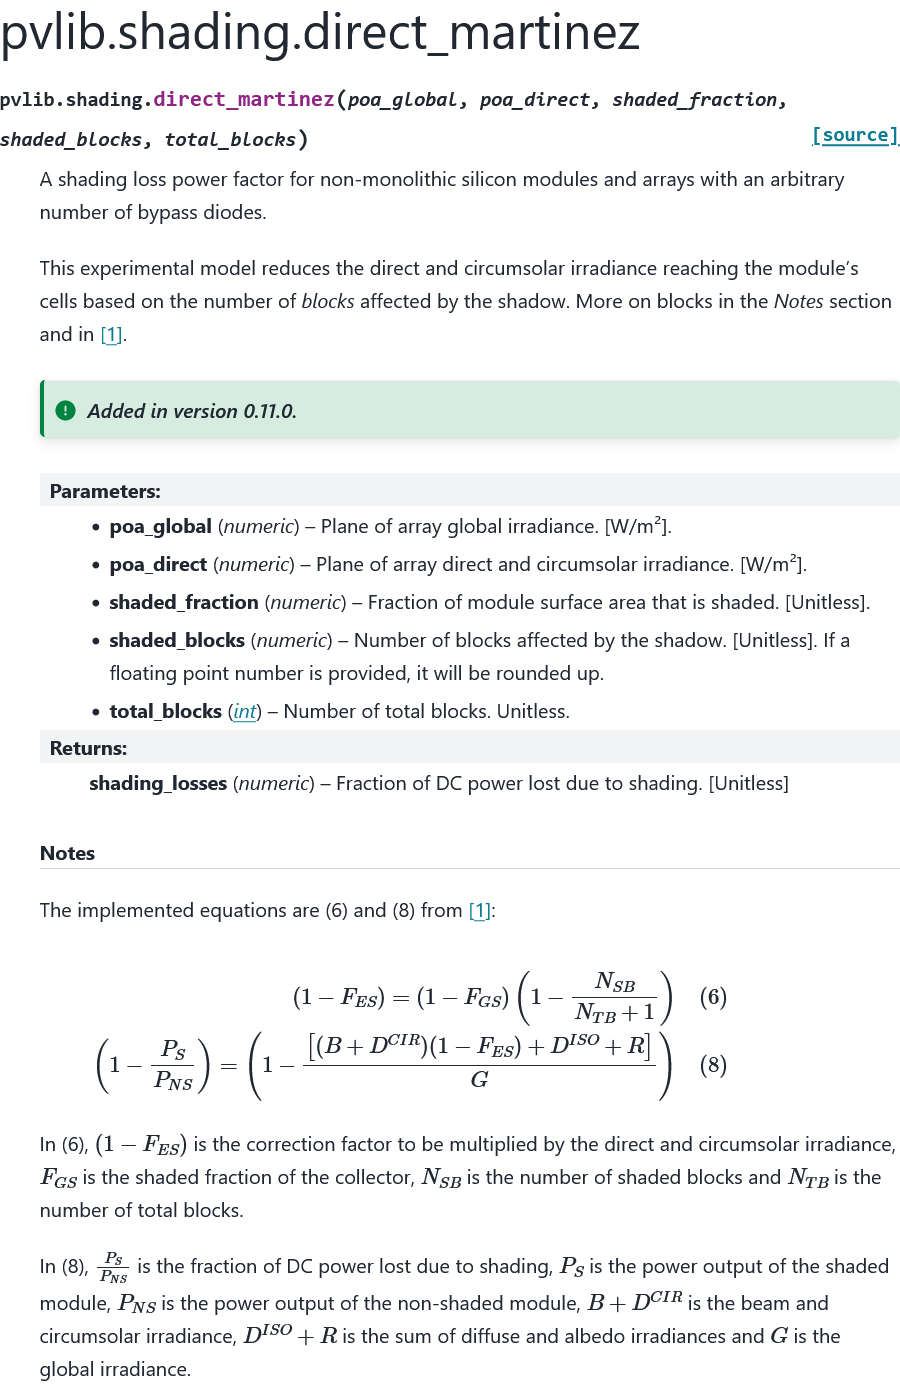
\includegraphics[width=\linewidth,height=0.9\textheight,keepaspectratio]{images/docs_funcs_cut/direct_martinez_0.png}

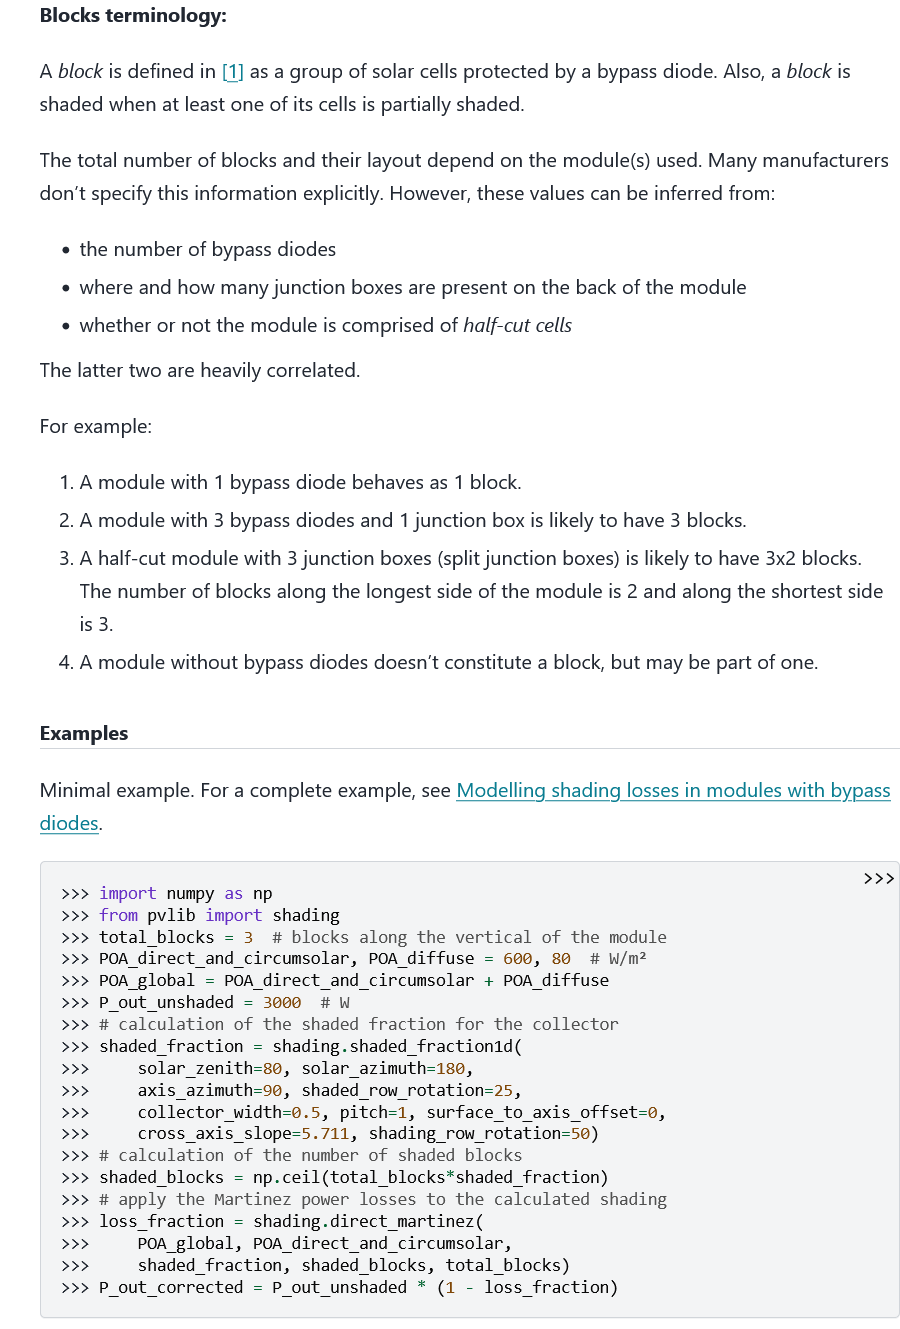
\includegraphics[width=\linewidth,height=0.9\textheight,keepaspectratio]{images/docs_funcs_cut/direct_martinez_1.png}

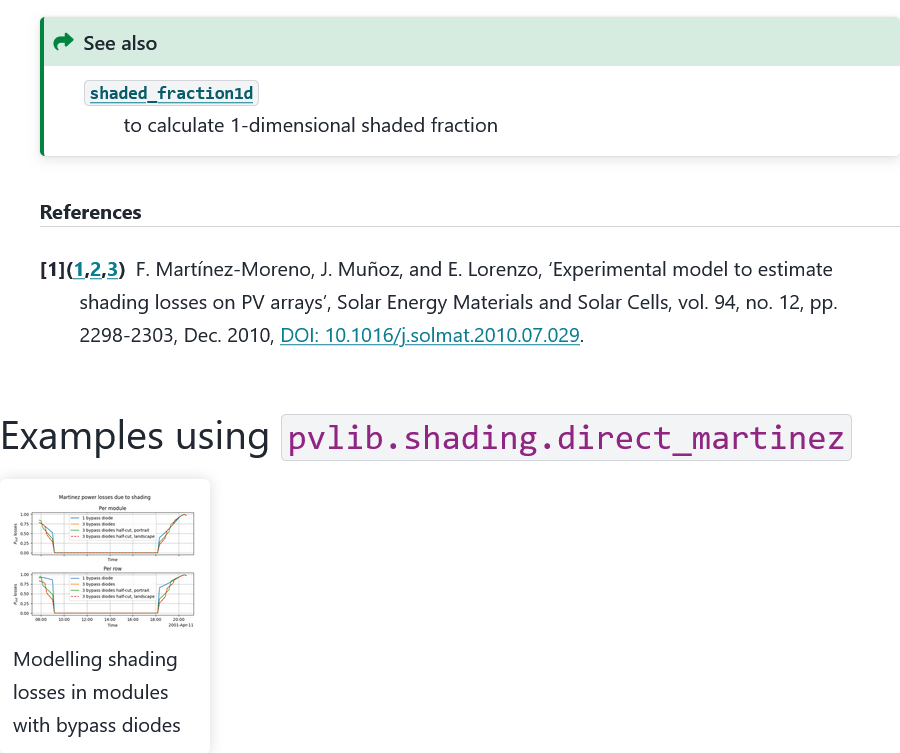
\includegraphics[width=\linewidth,height=0.9\textheight,keepaspectratio]{images/docs_funcs_cut/direct_martinez_2.png}

\newpage\section{Fracción difusa de radiación fotosintetizable diaria} \label{sct:doc_par_difusa}

\pr{2048}, accesible en \linkDocsFunction{pvlib.irradiance.diffuse\_par\_spitters}.

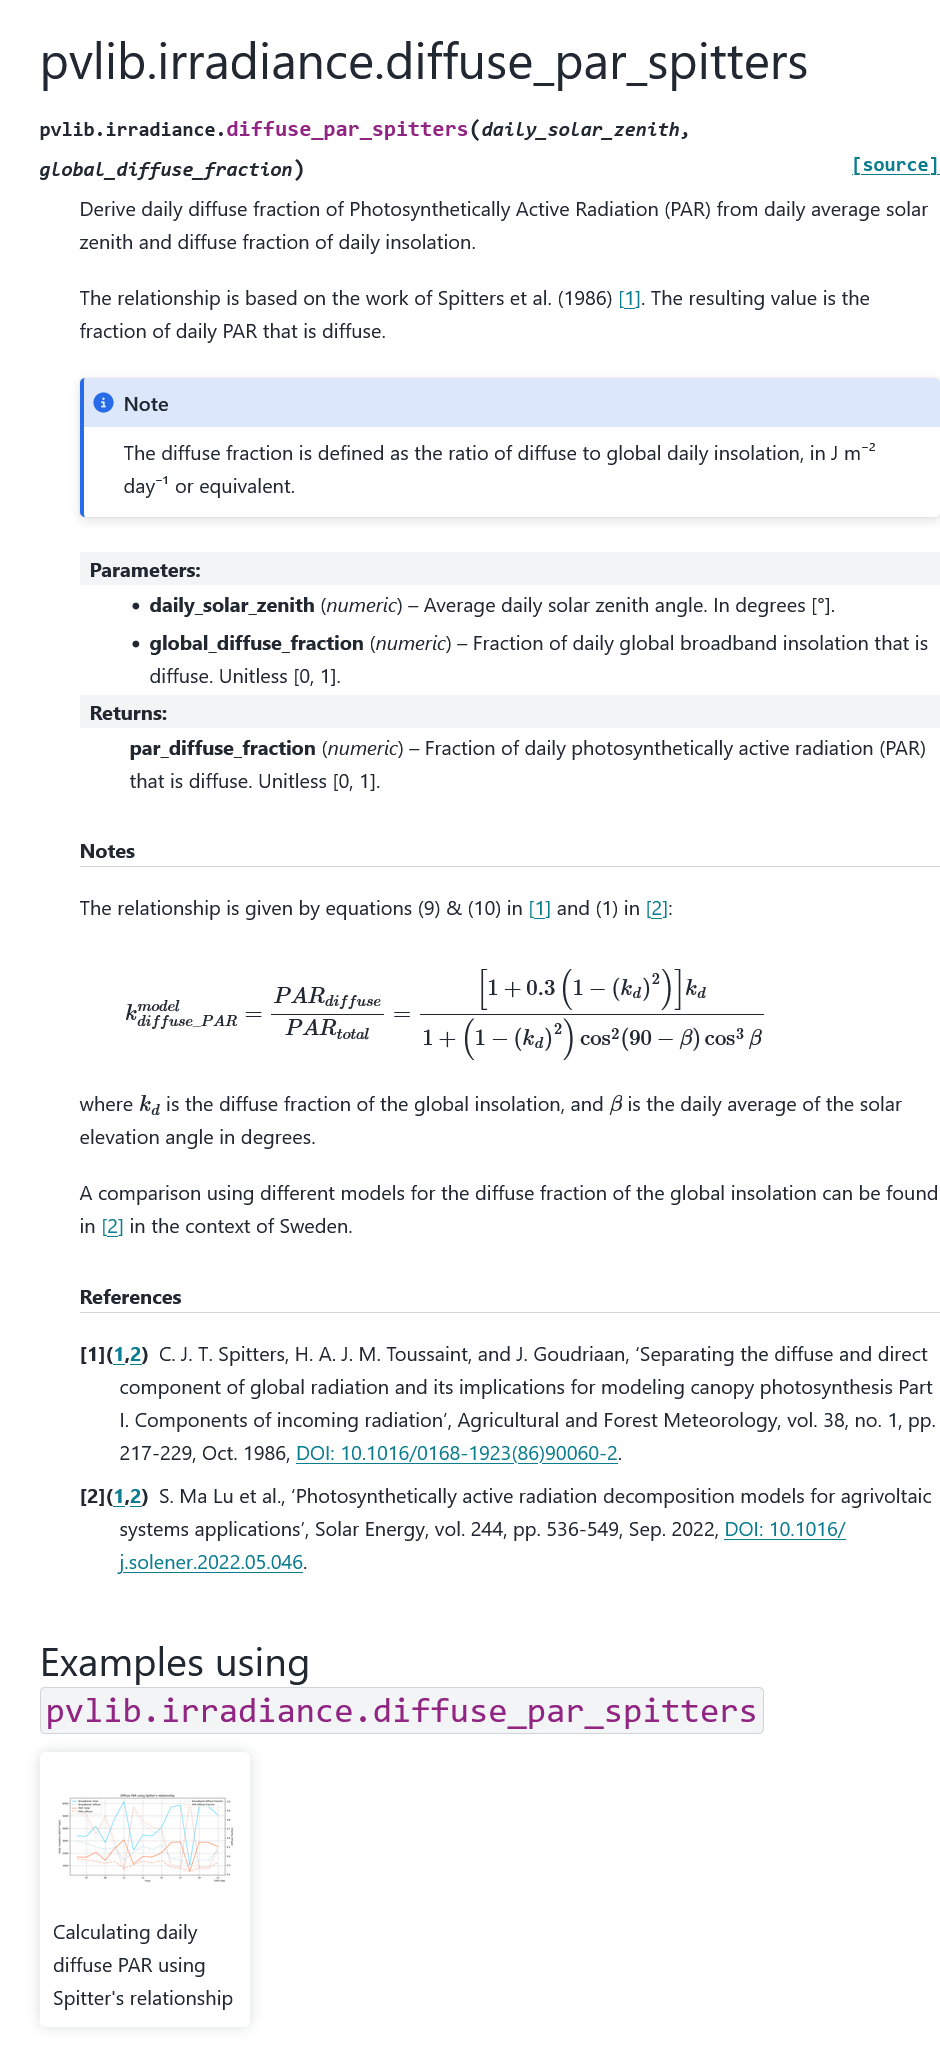
\includegraphics[width=\linewidth,height=0.9\textheight,keepaspectratio]{images/docs_funcs/pvlib.irradiance.diffuse_par_spitters.png}

\newpage\section{Modelo de pérdidas por irradiancia no uniforme} \label{sct:doc_modelo_ajuste_no_uniformidad}

\pr{2046}, accesible en \linkDocsFunction{pvlib.bifacial.power\_mismatch\_deline}.

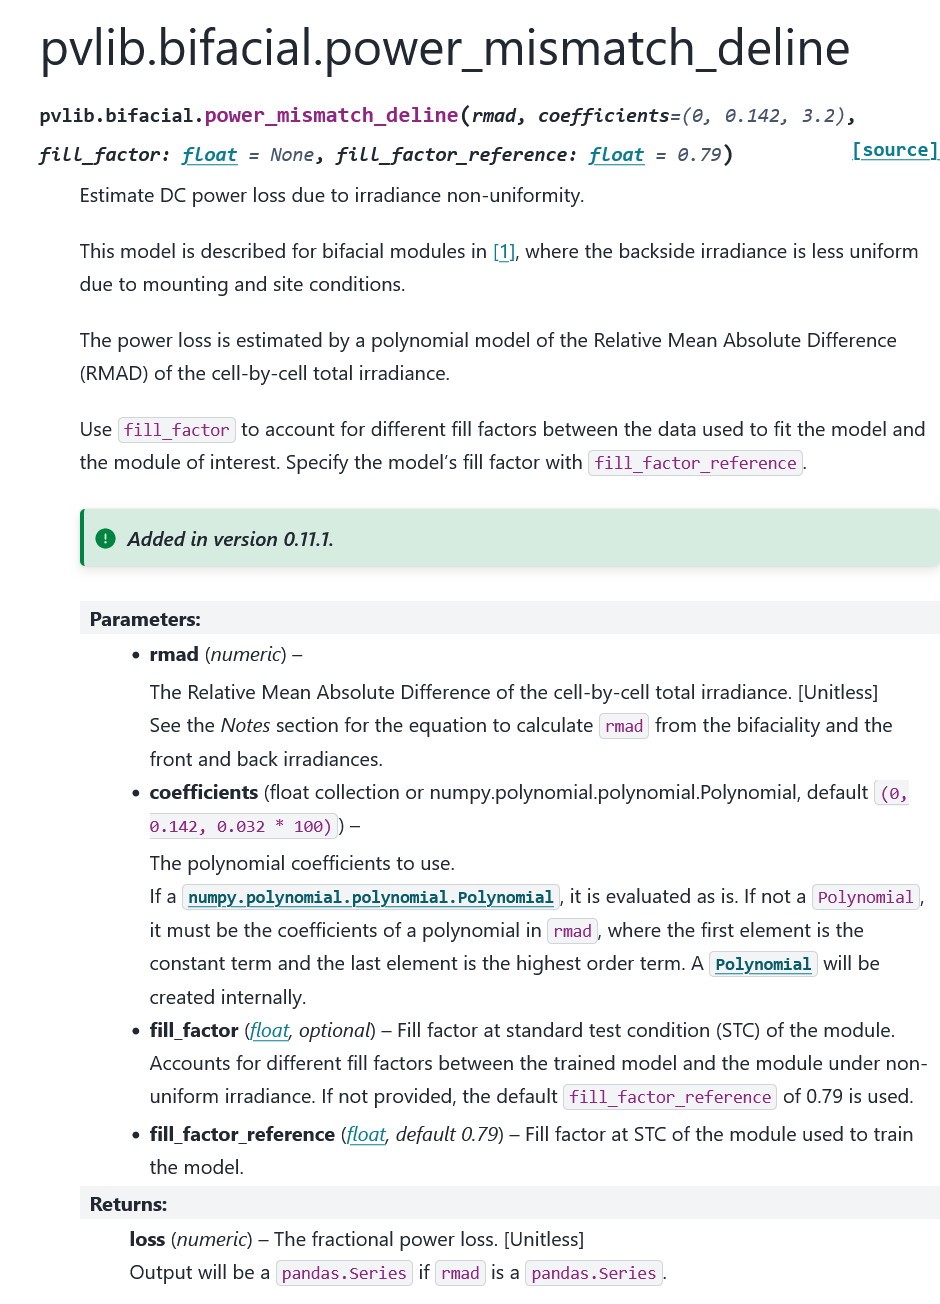
\includegraphics[width=\linewidth,height=0.9\textheight,keepaspectratio]{images/docs_funcs_cut/power_mismatch_deline_0.png}

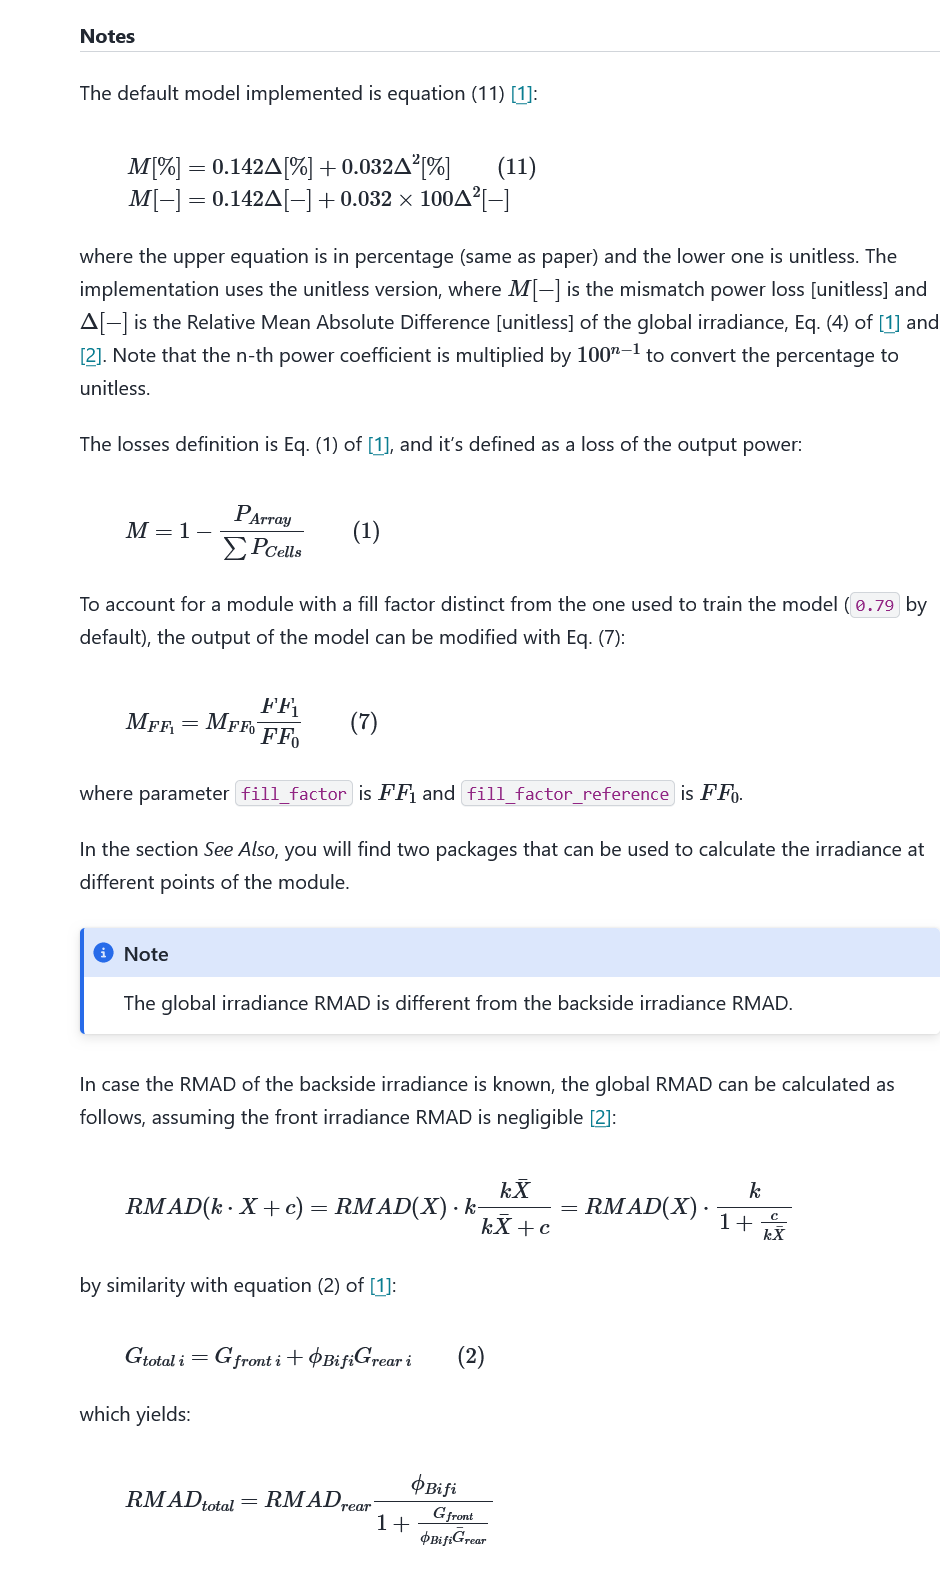
\includegraphics[width=\linewidth,height=0.9\textheight,keepaspectratio]{images/docs_funcs_cut/power_mismatch_deline_1.png}

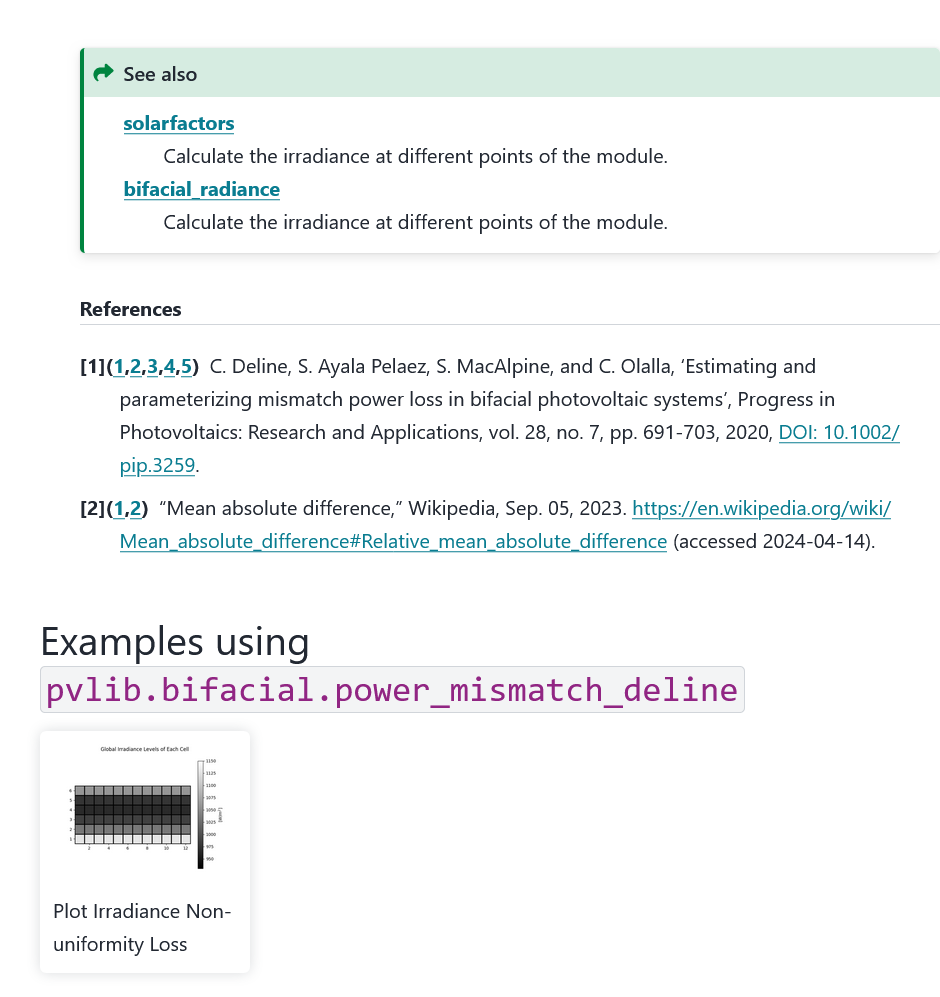
\includegraphics[width=\linewidth,height=0.9\textheight,keepaspectratio]{images/docs_funcs_cut/power_mismatch_deline_2.png}

\newpage\section{Conversión entre eficiencia cuántica y respuesta espectral} \label{sct:doc_sr_eq}

\pr{2041}, accesibles en \linkDocsFunction{pvlib.spectrum.qe\_to\_sr} y \linkDocsFunction{pvlib.spectrum.sr\_to\_qe}.

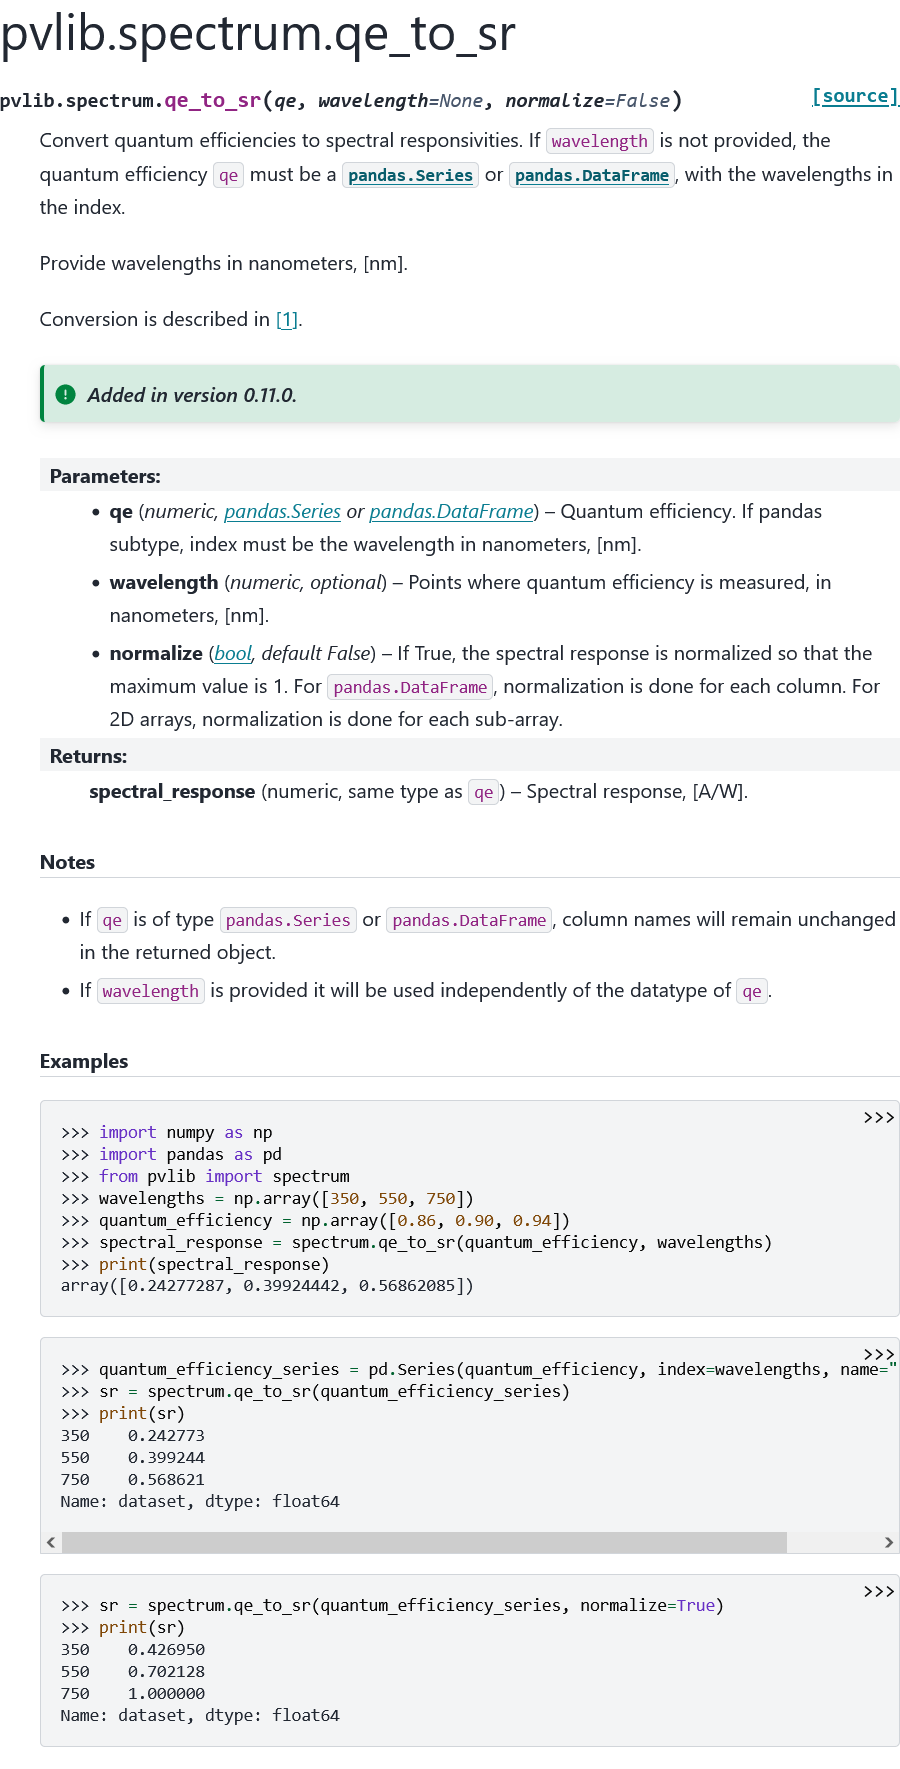
\includegraphics[width=\linewidth,height=0.9\textheight,keepaspectratio]{images/docs_funcs_cut/qe_to_sr_0.png}

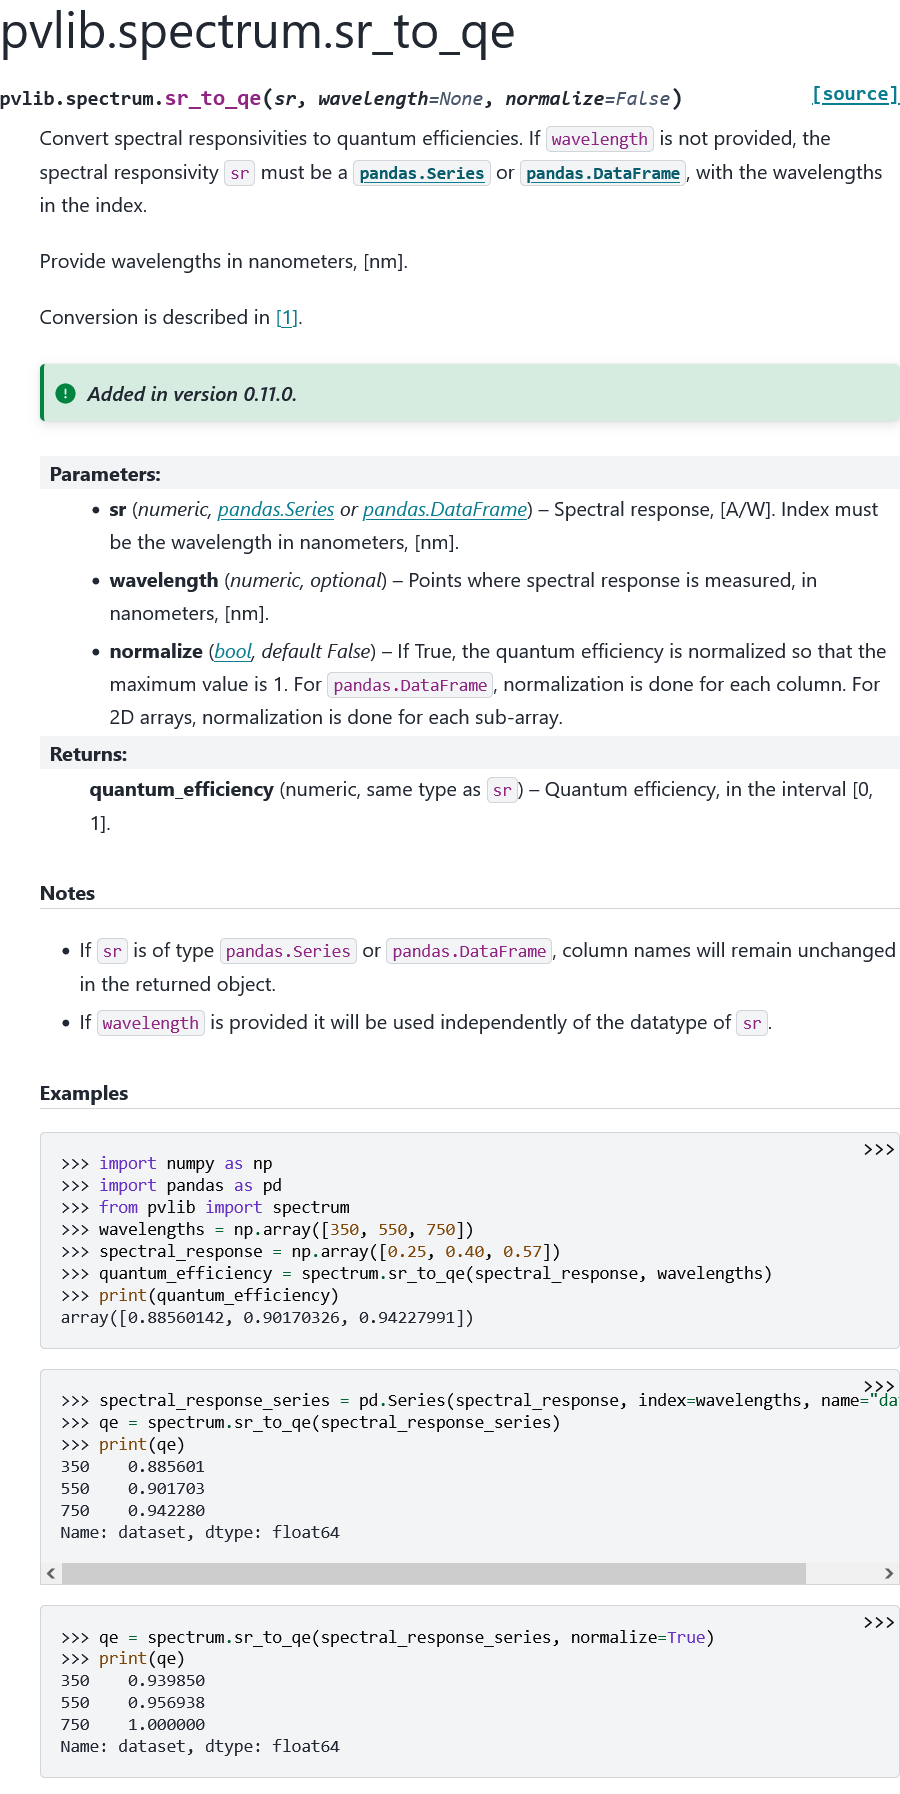
\includegraphics[width=\linewidth,height=0.9\textheight,keepaspectratio]{images/docs_funcs_cut/sr_to_qe_0.png}

\newpage\section{Espectro estándar ASTM G173-03} \label{sct:doc_espectro_astm-173-03}

\pr{1963}, accesible en \linkDocsFunction{pvlib.spectrum.get\_reference\_spectra}.

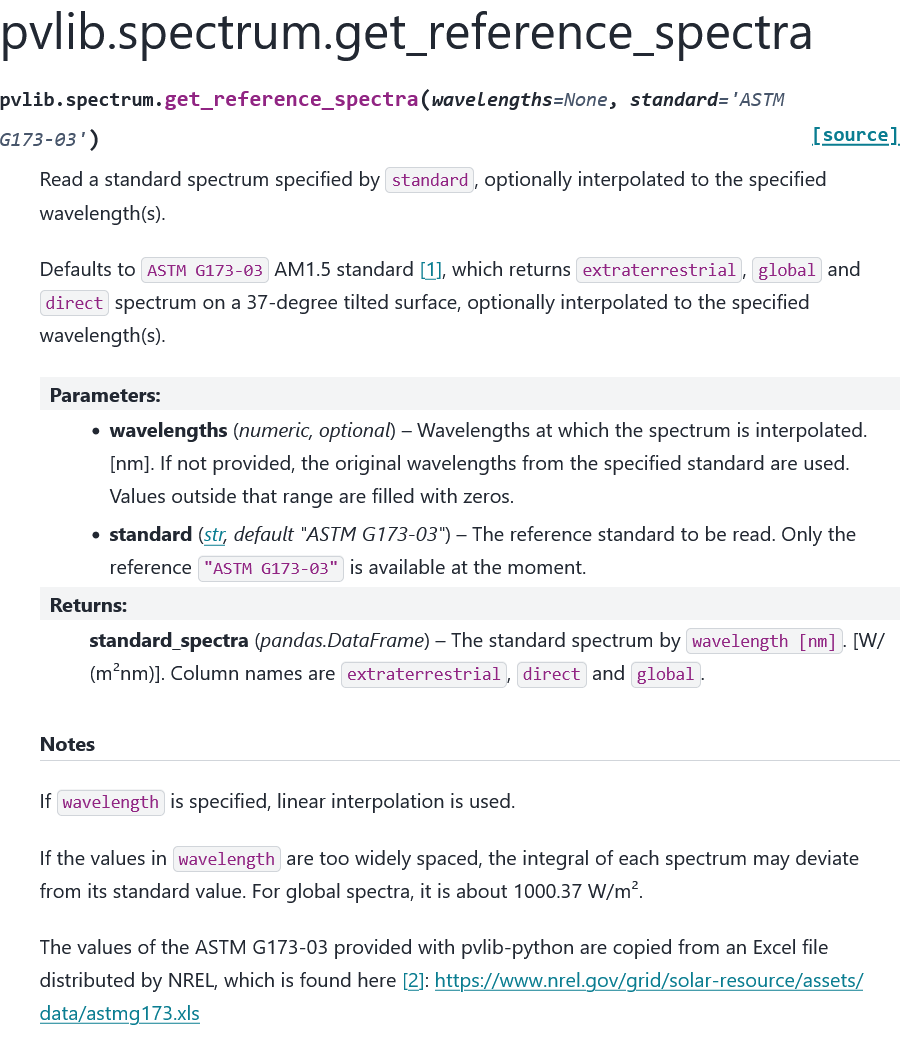
\includegraphics[width=\linewidth,height=0.9\textheight,keepaspectratio]{images/docs_funcs_cut/get_reference_spectra_0.png}

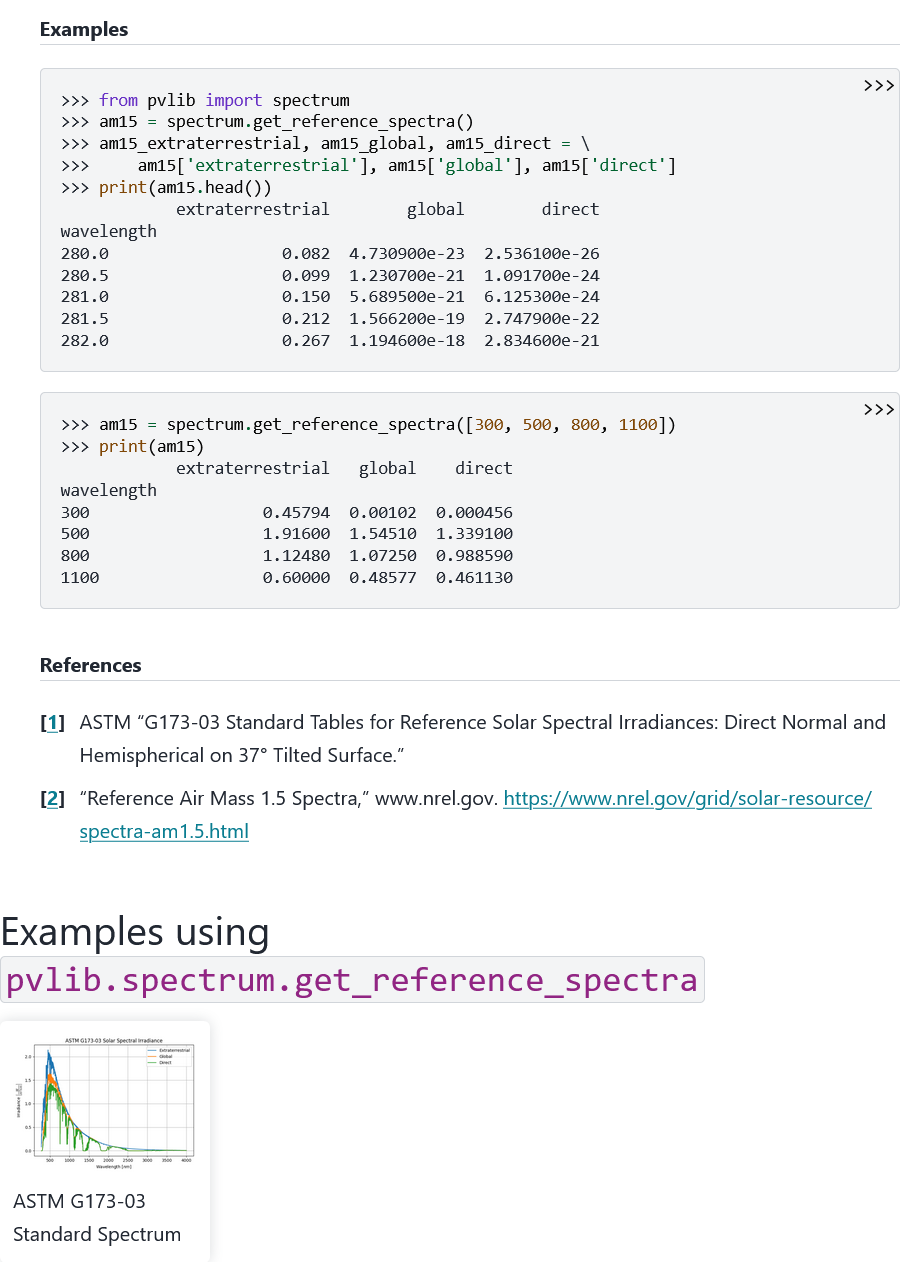
\includegraphics[width=\linewidth,height=0.9\textheight,keepaspectratio]{images/docs_funcs_cut/get_reference_spectra_1.png}

\newpage\section{Cálculo geométrico de sombras en 3D} \label{sct:doc_sombras_3d}

\pr{2106}, propuesta no aceptada, pero documentación disponible temporalmente en \href{https://pvlib-python--2106.org.readthedocs.build/en/2106/reference/generated/pvlib.spatial.FlatSurface.html}{pvlib.spatial.FlatSurface} y \href{https://pvlib-python--2106.org.readthedocs.build/en/2106/reference/generated/pvlib.spatial.RectangularSurface.html}{pvlib.spatial.RectangularSurface}.

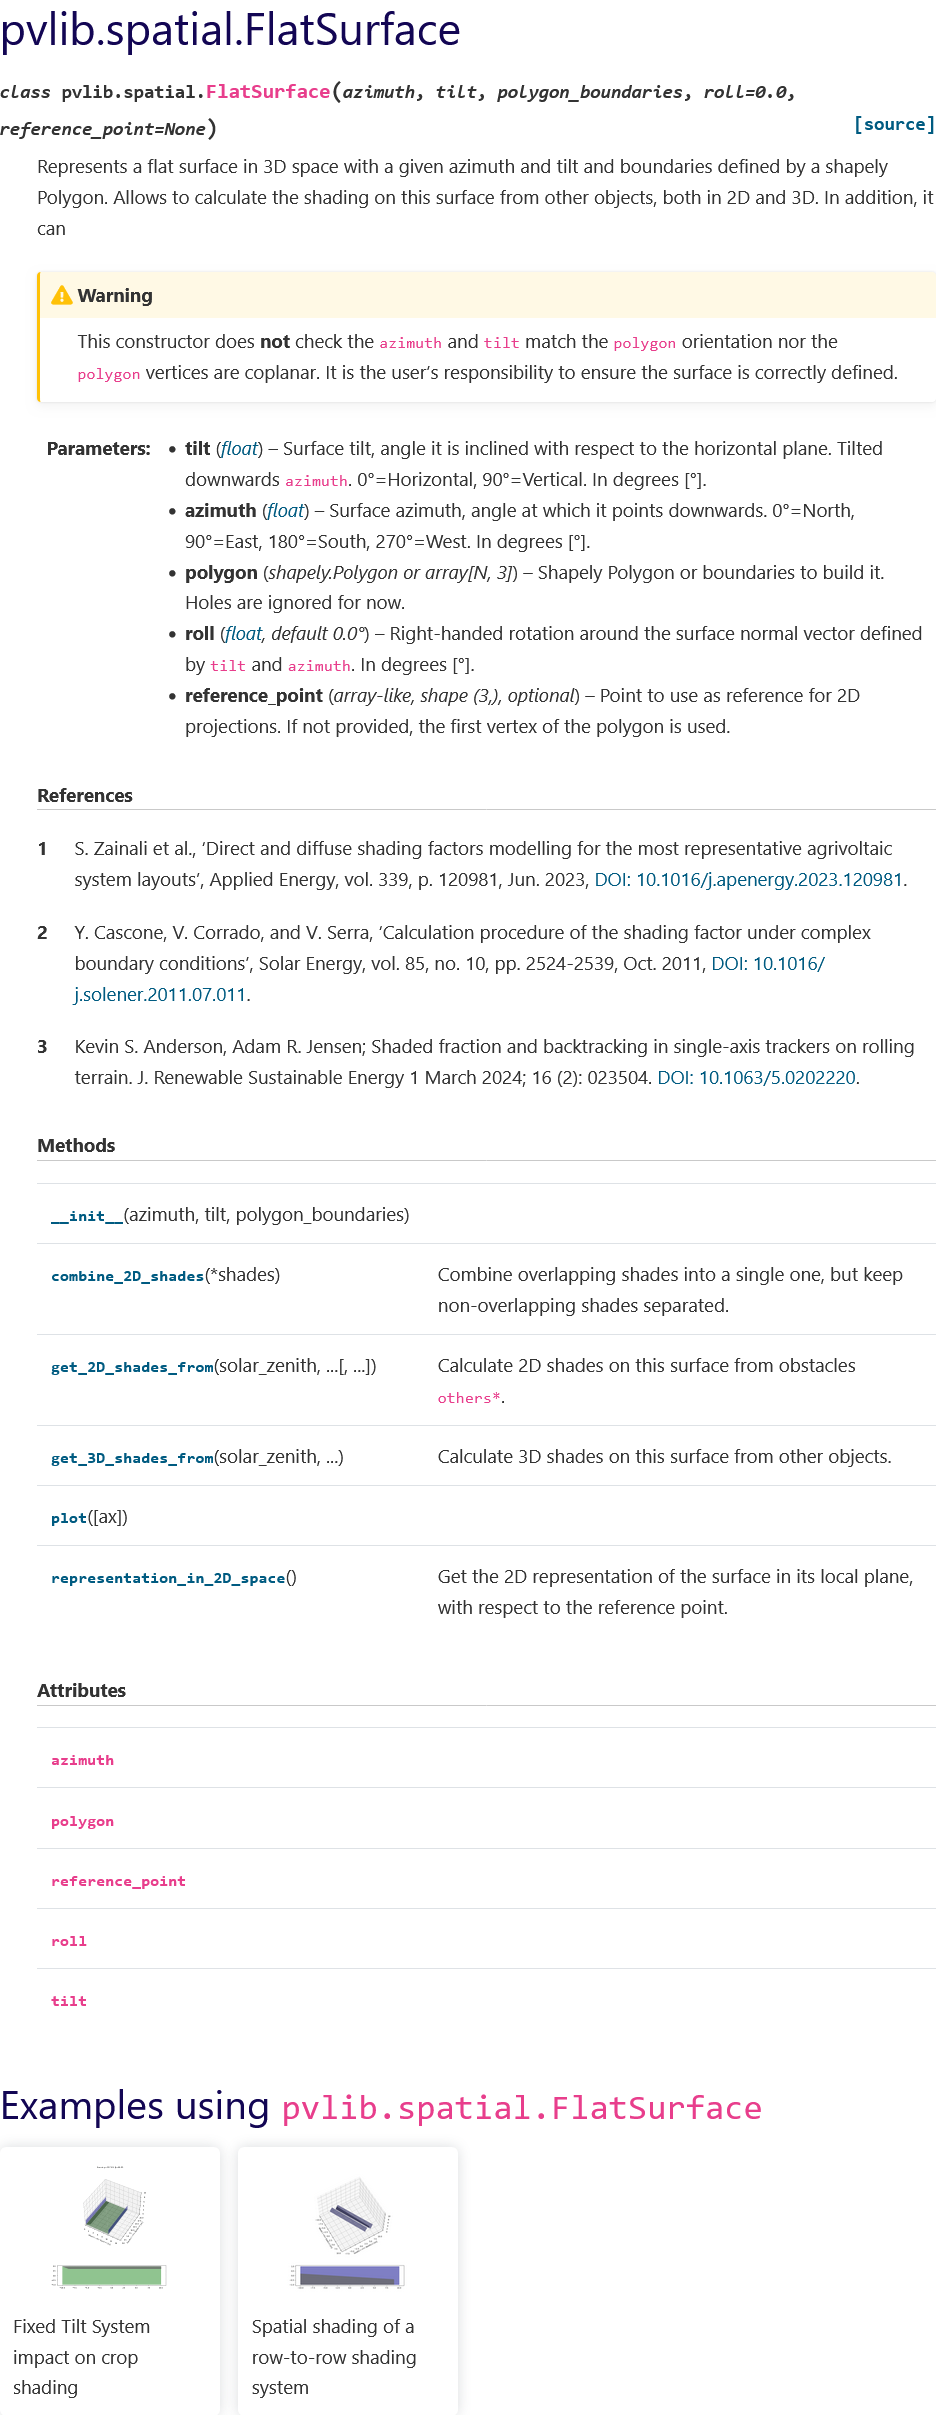
\includegraphics[width=\linewidth,height=0.9\textheight,keepaspectratio]{images/docs_funcs/pvlib.spatial.FlatSurface.png}

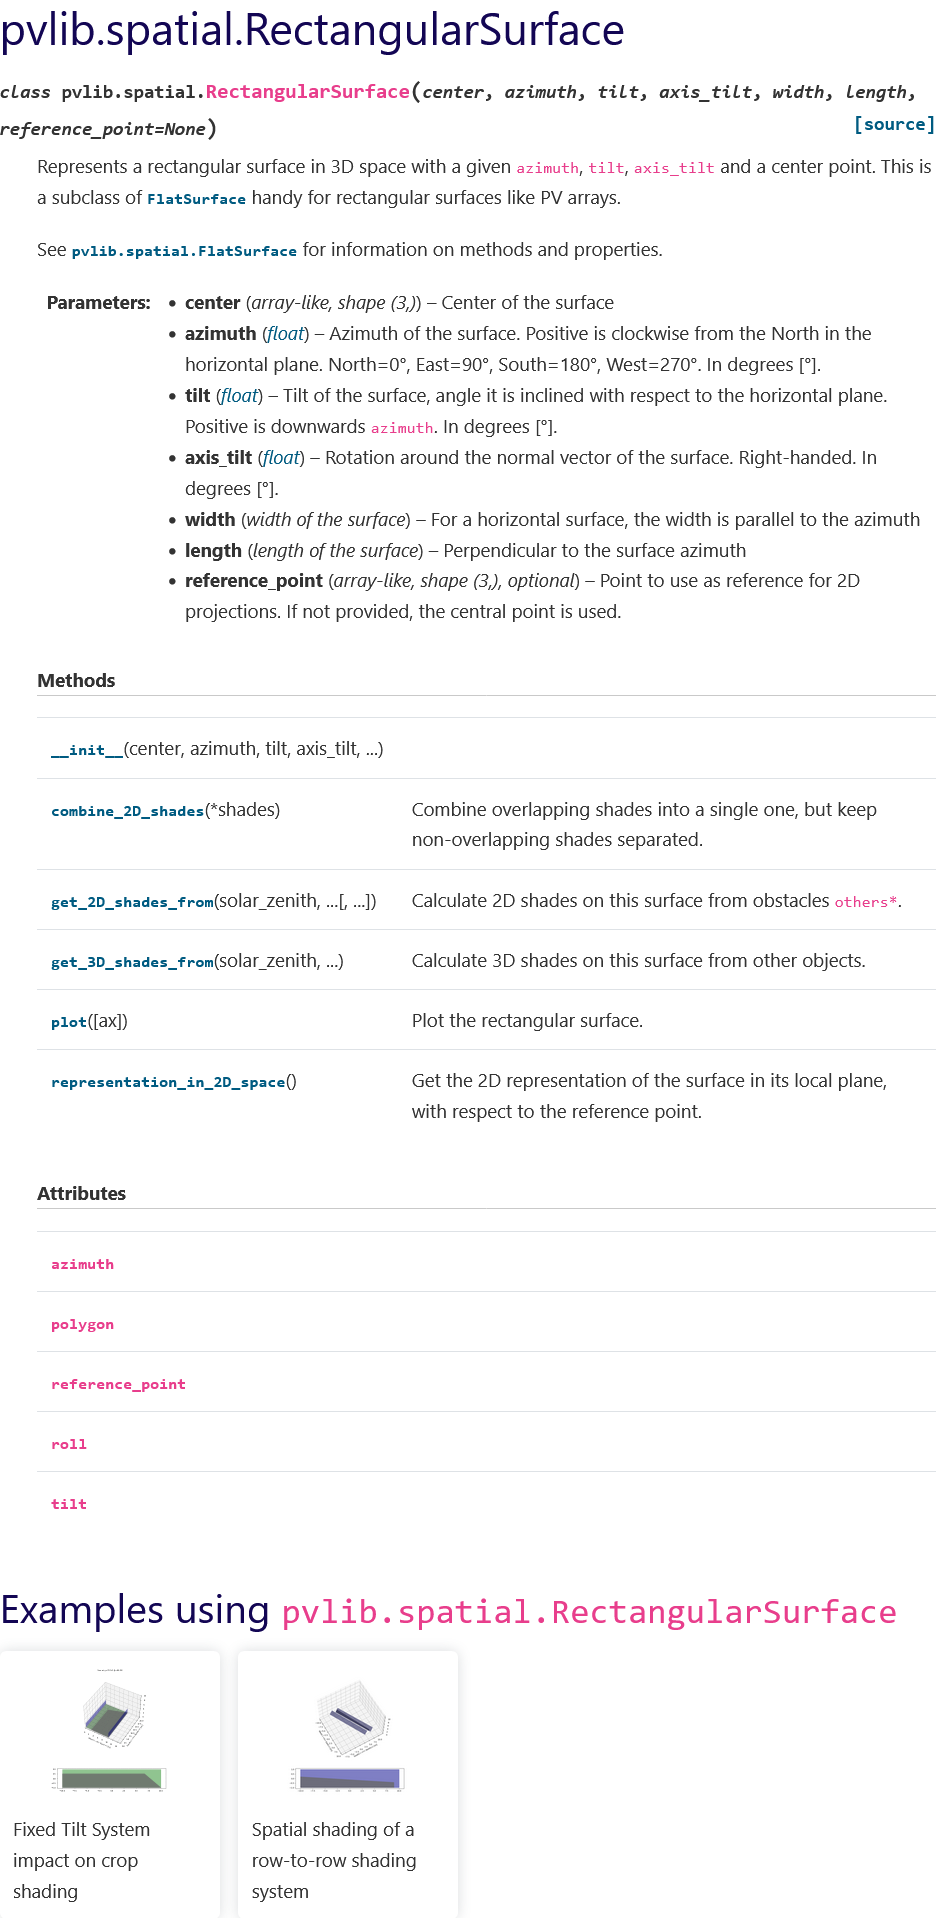
\includegraphics[width=\linewidth,height=0.9\textheight,keepaspectratio]{images/docs_funcs/pvlib.spatial.RectangularSurface.png}

%%%%%%%%%%%%%%%%%%%%%%%%%%%%%%%%%%%%%%%%%%%%%%%%%%%%%%%%%%%%%%%%%%%%%%%%%%%%%%%%
\end{myparindent}
